\section{The Sosiogram}
During the project the facilitators went around to the groups, analyzing how the communication within the team was during a discussion. They made a sosiogram of it by dotting down lines whenever someone talked to individuals or the group as a whole, as we can see in the sosiogram from our group, seen in \autoref{fig:sosiogram}. Note that when someone talked to the group in general, it's represented as a line towards the center dot of the "table".

What the group saw from the sosiogram was that the two people sitting on their laptop during the meeting, even though they were doing work relevant to the discussion, was much less active in the discussion. The group decided that this was something we didn't want, so from now on every meeting was pc-free, unless someone was specifically asked to either take notes as a secretary, or check something that we would need in the discussion.

In retrospect this helped make everyone active in the discussions, since we also saw from the sosiogram that everyone was about as active as the others, with the exception of those using their laptop. 
\newpage{}
\begin{figure}
	\begin{center}
		\frame{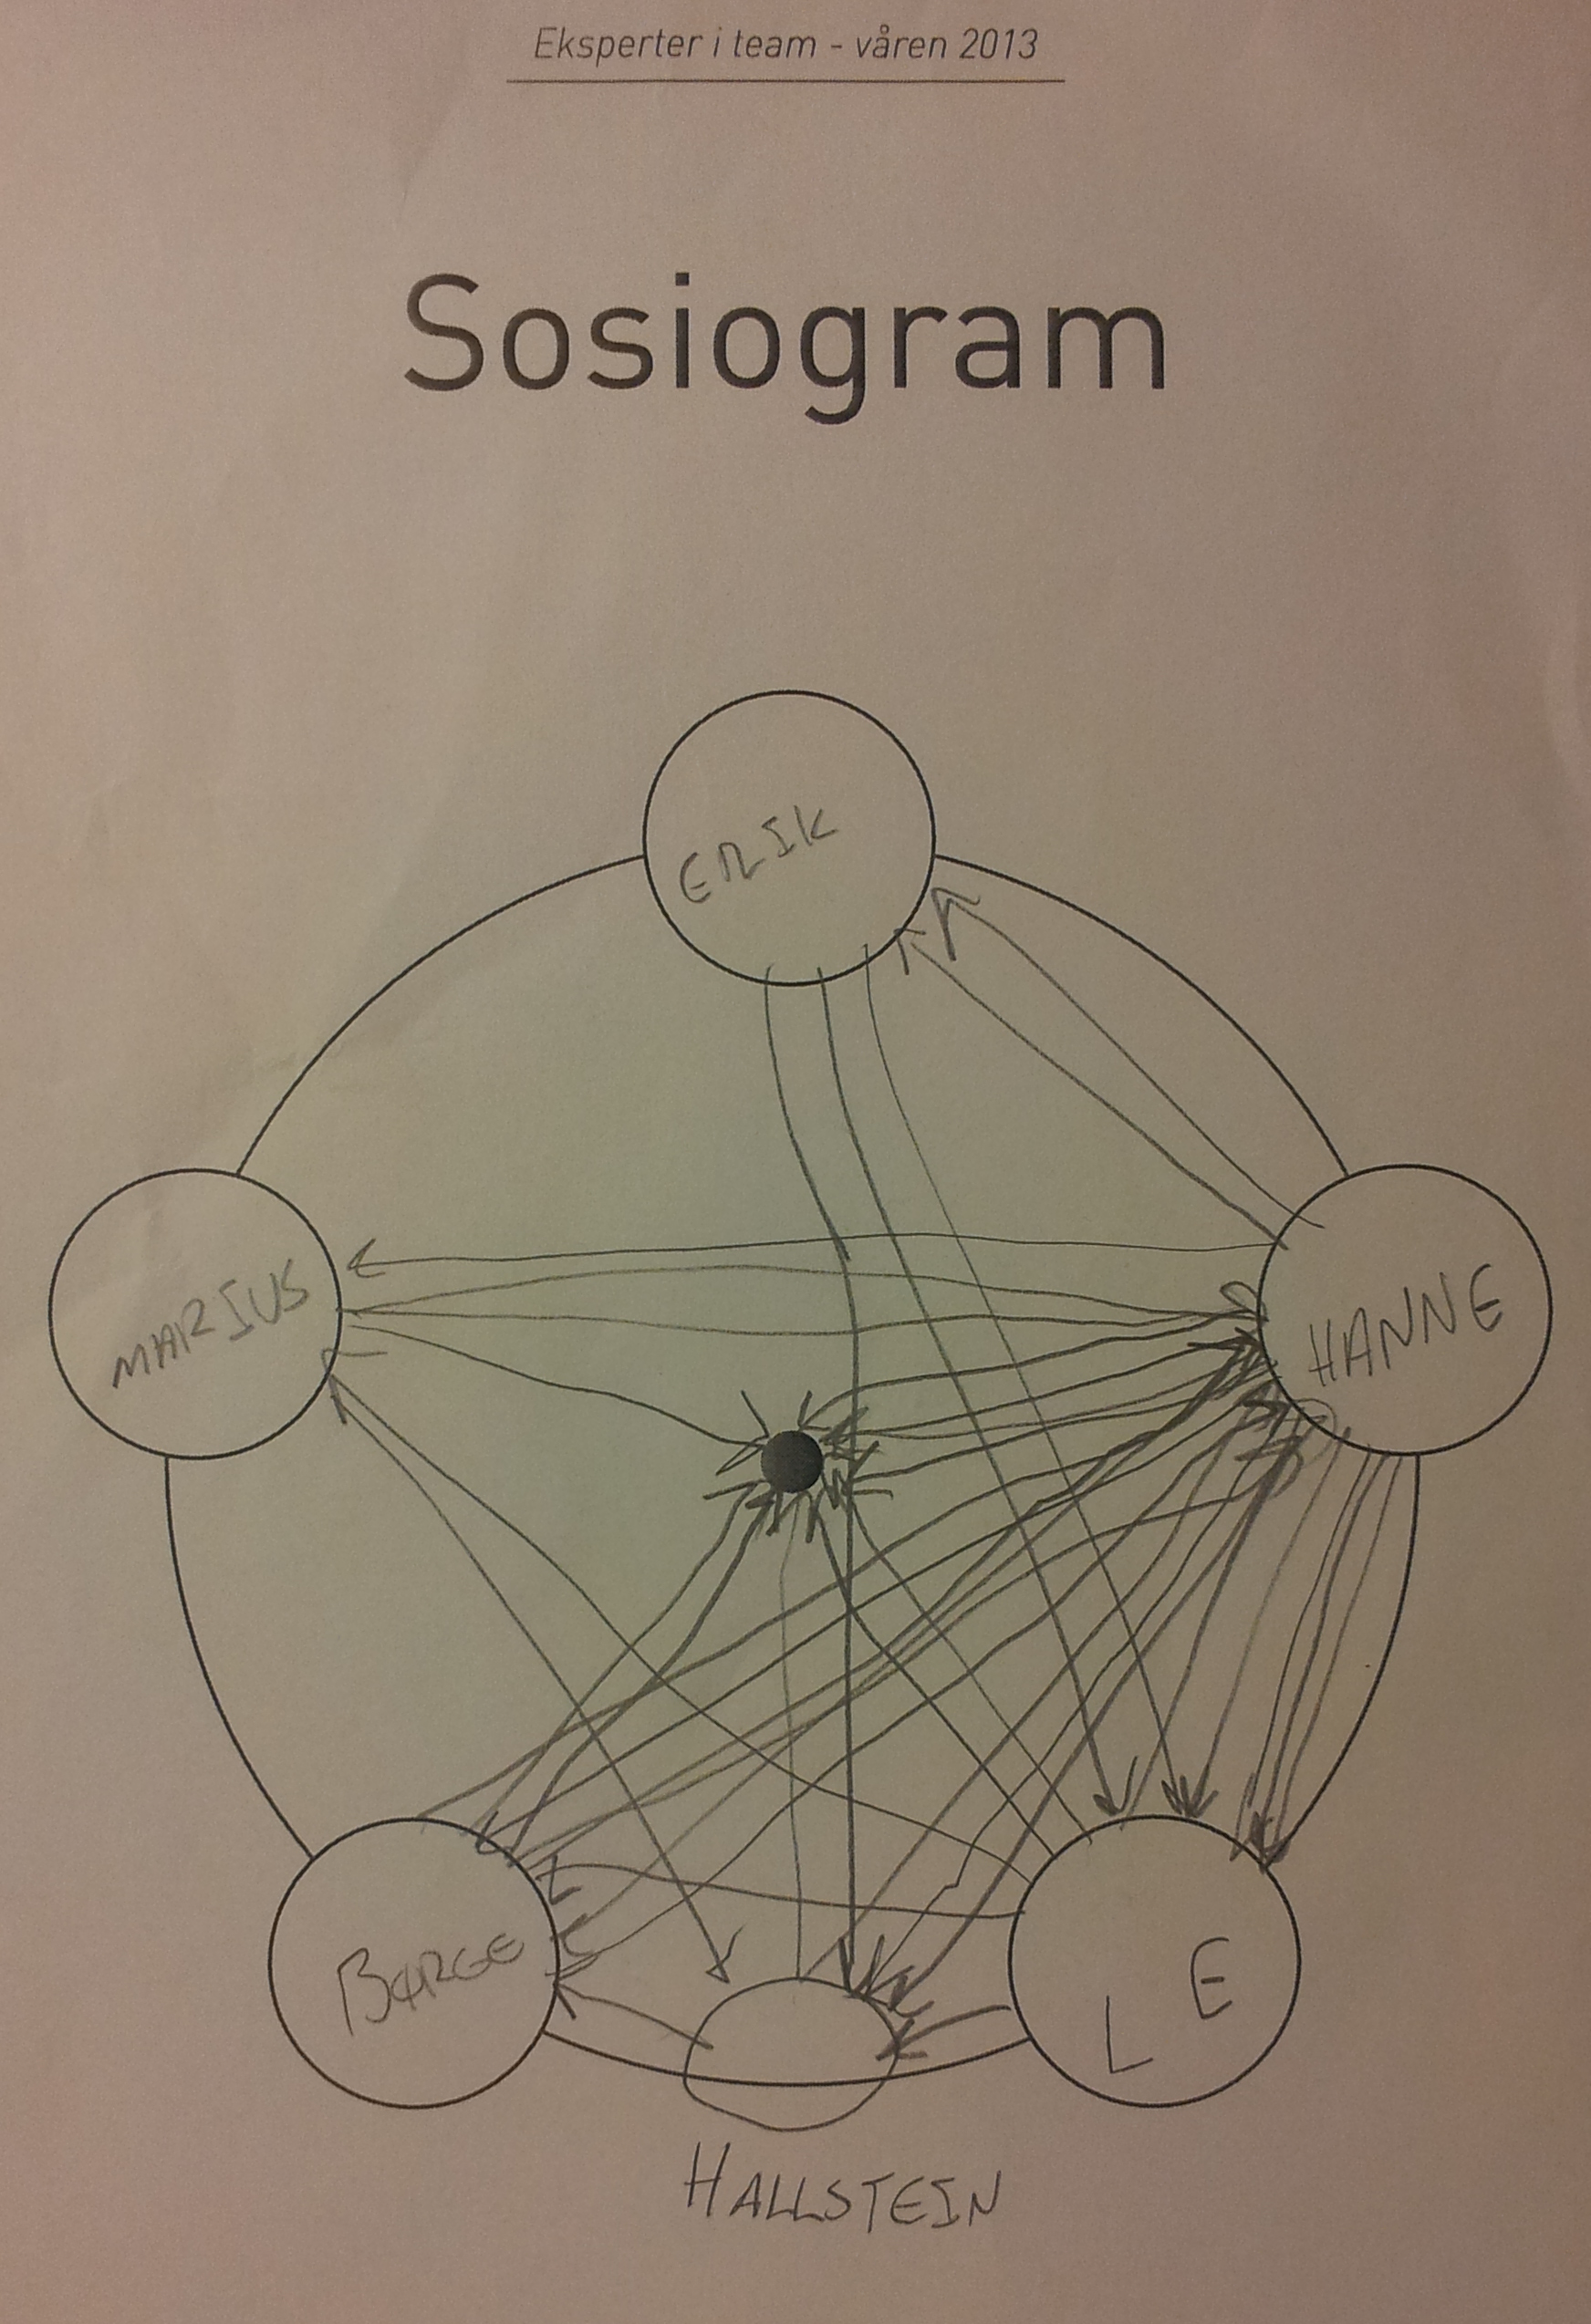
\includegraphics[width=0.7\textwidth]{Figures/sosiogram.png}}
	\end{center}
	\caption[The Sosiogram]{The Sosiogram we got from the facilitators after they observed a discussion in the group}
	\label{fig:sosiogram}
\end{figure}